
\chapter{\IfLanguageName{dutch}{Wetgeving omtrent nummerplaatdetectie}{Technical details about ANPR in the GDPR}}
\label{ch:wetgeving-nummerplaatdetectie}

Het is vanzelfsprekend dat er enkele wetgevingen zijn die slaan op nummerplaatdetectie, het nemen van foto's als toegangssysteem is een pak meer privacyingrijpend dan een token in te werpen. Sinds de nieuwe wet van de GDPR in 2018 moet hier dan ook veel voorzichtiger met worden omgegaan.

In de volgende onderdelen wordt er beschreven wat deze wet inhoudt en op welke manier nummerplaatdetectie hieronder valt.

\section{Algemene verordening gegevensbescherming}
%Wanneer is gdpr van toepassing
De General Data Protection Regulation (GDPR) of in het Nederlands: Algemene Verordening Gegevensbescherming (AVG), is een nieuwe wetgeving die op 25 mei 2018 ingevoerd is met als doel regels op te stellen om de grondrechten en de fundamentele vrijheden van natuurlijke personen te beschermen in de Europese Unie, dit met name op hun recht op bescherming van persoonsgegevens. \autocite{avg2018privacy}

Voor de verwerking van deze gegevens worden maatregelen opgelegd over hoe deze op een correcte manier behandeld moeten worden en aan welke eisen een bedrijf moet voldoen indien deze hiermee handeld.

In dit onderdeel zal niet de volledige AVG beschreven worden, maar enkel de onderdelen m.b.t. een parkeersysteem met nummerplaatdetectie.

\subsection{Definities}

\paragraph{Persoonsgegevens}
In artikel 4 van het AVG worden persoonsgegevens als volgt beschreven: 'alle informatie over een geïdentificeerde of identificeerbare natuurlijke persoon ("de betrokkene"); als identificeerbaar wordt beschouwd een natuurlijke persoon die direct of indirect kan worden geïdentificeerd, met name aan de hand van een identificator zoals een naam, een identificatienummer, locatiegegevens, een online identificator of van een of meer elementen die kenmerkend zijn voor de fysieke, fysiologische, genetische, psychische, economische, culturele of sociale identiteit van die natuurlijke persoon' \autocite{avg2018privacy}

Hieruit blijkt dat nummerplaten onder de term persoonsgegevens vallen; Deze zijn geregistreerd aan een persoon en kunnen worden gebruikt om de persoon te identificeren. In een parkeersysteem met nummerplaatdetectie zal hier dus ook op gelet moeten worden. 

Artikel 5 van GDPR, 'persoonsgegevens moeten worden verwerkt op een wijze die ten aanzien van de betrokkene rechtmatig, behoorlijk en transparant is ("rechtmatigheid, behoorlijkheid en transparantie")` \autocite{avg2018privacy}.

\paragraph{Betrokkene}
De betrokkene is een geïdentificeerde of identificeerbare natuurlijke persoon wie de vermelde persoonsgegevens bezit.

\paragraph{Verwerking van gegevens}
Een verwerking is een veel vermelde term in het AVG en omvat een duidelijke definitie. Het verwerken van gegevens omvat eender welke operaties die op persoonsgegevens worden uitgevoerd. Waaronder het verzamelen, vastleggen, organiseren, raadplegen of vernietigen van deze gegevens onderdeel van is. Deze lijst wordt verder uitgebreid omschreven in Artikel 4 punt 2 van de GDPR.

Indien een ANPR-systeem foto's neemt van auto's dan voert deze enkele verwerkingen uit. Deze zijn het vastleggen, raadplegen en mogelijks vernietigen van de gegevens. Ookal duurt dit proces maar enkele seconden en wordt er niets opgeslaan is er wel degelijk sprake van een verwerking.

\paragraph{Verwerkingsverantwoordelijke}
De verwerkingsverantwoordelijke is een persoon die instaat voor het correct verwerken van gegevens. Hij bepaalt het doel en de middelen van de verwerking. Op vraag van overheidsinstanties moet hij kunnen aantonen waarom en hoe de verwerking wordt uitgevoerd.

\paragraph{Verwerker}
Een verwerker is een persoon die persoonsgegevens verwerkt in opdracht van de verwerkingsverantwoordelijke.

\subsection{Beginselen inzake gegevensverwerking}
Het is niet mogelijk om zomaar welke persoonsgegevens te verwerken. De GDPR stelt enkele regels op die organisaties moeten naleven voor het verwerken van gegevens. De verwerkingsverantwoordelijke moet kunnen aantonen dat deze nageleefd worden. De beginselen inzake gegevensverwerking zijn te vinden in Artikel 5 van de GDPR.

\paragraph{Rechtmatigheid van verwerking}
\label{rechtmatigheid-van-verwerking}
Een verwerking van persoonsgegevens dient ten alle tijden rechtmatig te zijn, indien dit niet het geval is kunnen er sancties optreden.

In artikel 6 beschrijft de GDPR enkele voorwaarden waar minstens aan voldaan moet worden. Zo kan de betrokkene toestemming gegeven hebben, is er een wettelijke plicht of zijn er gerechtvaardigde belangen voor de verwerking van de gegevens.

In het geval van een ANPR-camera is het niet mogelijk om toestemming aan de betrokkene te vragen. Dit omdat toevallige voorbijgangers ook de camera kunnen triggeren welke vervolgens hun gegevens verwerkt, waarvoor deze geen toestemming hebben kunnen geven. Hiervoor is de enige echte optie het gerechtvaardigd belang.

Het gerechtvaardigd belang berust erop dat de belangen van de verwerking meer doorwegen dan de belangen van de betrokkene. En dat dit belang enkel kan behartigd worden door persoonsgegevens te verwerken \autocite{autoriteit2019gerechtvaardigd}.

\paragraph{Doelbinding}
De doeleinden voor de gegevensverwerking dienen uitdrukkelijk omschreven en gerechtvaardigd te zijn. Geen verdere verwerking is toegestaan die niet aan deze doeleinden beantwoordt.

\paragraph{Dataminimalisatie en juistheid}
De opgeslagen data dienen beperkt te zijn tot wat nodig is om de beschreven doeleinden te voldoen. Het is de bedoeling om een strikt minimum van data bij te houden. Verder moet de data actueel gehouden worden en indien onjuist, verwijdert of gerectificeerd te worden.

\paragraph{Opslagbeperking}
Indien de betrokkene identificeerbaar is, mag de data niet langer opgeslaan worden dan dat deze nodig is voor het verwezenlijken van de doeleinden.

\paragraph{Integriteit en vertrouwelijkheid}
De verwerking dient genoeg beveiligd te zijn door gebruik te maken van passende, technische organisatorische maatregelen. Verder dient deze beschermd te zijn tegen iedere niet toegelate of onwettige verwerking, tegen verlies, vernietiging of kwaliteitsverlies van de gegevens.

\paragraph{Verantwoordingsplicht}
De verwerkingsverantwoordelijke is verantwoordelijk voor de naleving van deze beginselen van de verordening. Hij moet kunnen dan ook ten alle tijde kunnen aantonen dat aan deze beginselen voldaan zijn.


\subsection{Rechten van de betrokkene}
\label{rechten-betrokkene}
Vervolgens stelt de GDPR enkele uitgebreide rechten op die de betrokkene, de eigenaar van de persoonsgegevens, heeft. Deze zijn terug te vinden in hoofdstuk III van de GDPR en zijn omschreven in de volgende punten.

\paragraph{Recht om geïnformeerd te zijn}
Indien een ANPR-systeem is opgesteld, dient er volgens artikel 13 van de GDPR, gesignaleerd te worden dat een dergelijk systeem aanwezig is, dit tesamen met contactinformatie van de verwerkingsverantwoordelijke, de verwerkingsdoeleinden waarvoor de persoonsgegevens zijn bestemd en de rechtsgrond van de verwerking. Een voorbeeld van zo'n signalisatie is te zien in Figuur \ref{anpr-aanduiding}.

Deze signalisatie moet vanaf een duidelijke afstand zichtbaar zijn zodat de betrokkene deze kan lezen vooraleer hij de gemonitorde omgeving betreedt. Deze omgeving moet duidelijk zijn voor de betrokkene zodat hij deze kan mijden.

\begin{figure}[h!]
	\centering
	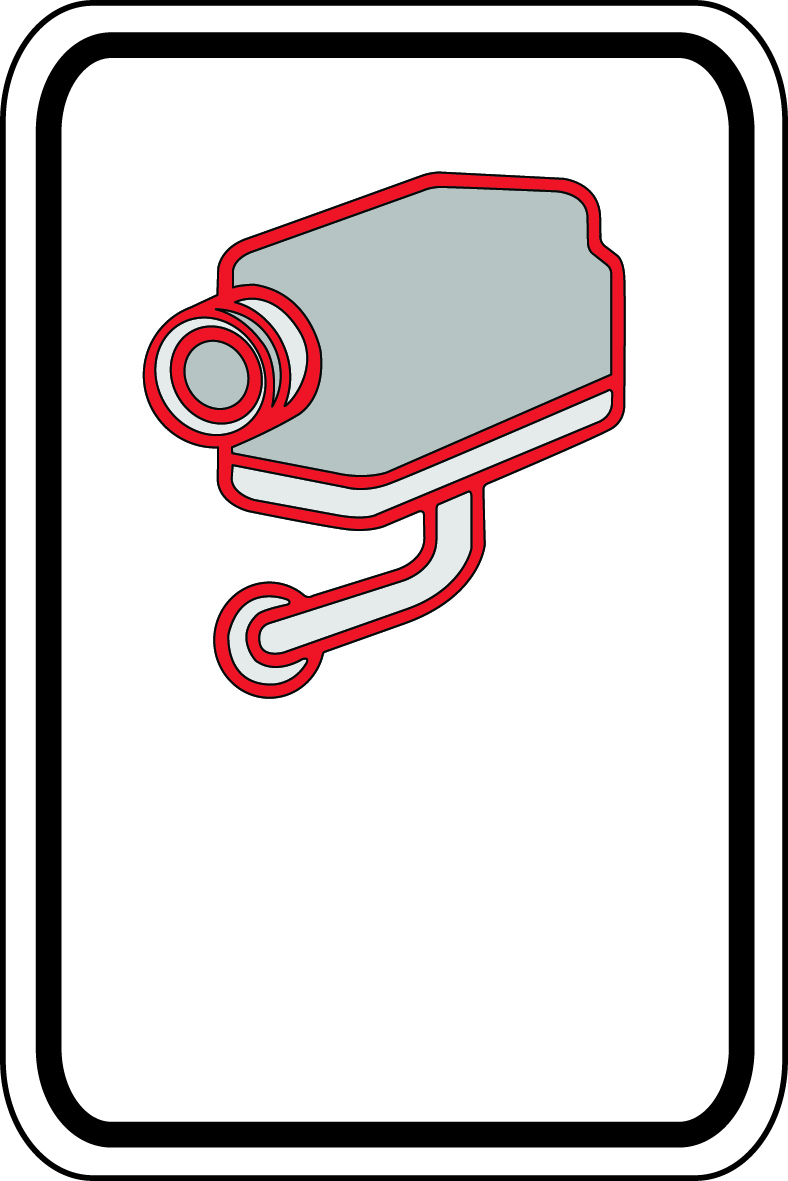
\includegraphics[width=\linewidth]{img/anpr-aanduiding.png}
	\caption{Voorbeeld van camerasignalisatie \autocite{edpb2019guidelines}}
	\label{anpr-aanduiding}
\end{figure}

\paragraph{Recht op informatie en rectificatie van persoonsgegevens} 
Iedereen bezit zijn eigen persoonlijke data en mag deze bijgevolg ook inkijken en corrigeren. Indien een gebruiker vraagt om zijn persoonsgegevens in te kijken, moet het bedrijf in kwestie al de persoonsgegevens van de gebruiker binnen de maand kunnen opleveren. Ook kan een gebruiker op eender wanneer beslissen om al zijn data te laten verwijderen \autocite{avg2018privacy}. Dit is terug te vinden in artikel 15 en 16 van de GDPR.

\paragraph{Recht op vergetelheid}
Een verwerkingsverantwoordelijke is verplicht persoonsgegevens zonder onredelijke vertraging te wissen indien deze niet meer nodig zijn voor de oorspronkelijke doeleinden, de gegevens onrechtmatig verwerkt zijn of de betrokkene zijn toestemming intrekt. Enkel indien één van de uitzonderingen in artikel 17 (3) van toepassing zijn kan dit langer duren. \autocite{edpb2019guidelines}

\paragraph{Recht op beperking van verwerking}
Bij camerasystemen die berusten op het gerechtvaardigd belang of openbaar belang om data te verwerken, heeft een betrokkene het recht om op eender welk moment hier bezwaar op te maken. Indien de verwerkingsverantwoordelijke geen legale gronden kan voorleggen die zwaarder doorwegen dan de rechten van de betrokkene, is hij verplicht aan de wensen van de betrokkene te voldoen. Dit is terug te vinden in artikel 18 van de GDPR.

In een context van camerabewaking kan deze objectie gemaakt worden voor, tijdens, of na een betrokkene een bewaakte zone betreedt. Dit betekent dat indien de belangen van de verwerkingsverantwoordelijke niet doorwegen tot de rechten van de betrokkene, de camera direct moet kunnen stopgezet worden van de betrokkene zijn data te kunnen verwerken. Anderzijds is het ook mogelijk om de gemonitorde zone genoeg af te bakenen zodat de verwerkingsverantwoordelijke de toestemming kan verifieren alvorens de betrokkene deze betreedt. \autocite{edpb2019guidelines}

%\subsection{Data Protection Officer}
%Een Data Protection Officer (DPO) moet aangesteld worden, Nederlands: Functionaris voor gegevensbescherming. NIET NODIG VOOR KLEINE ORGANISATIE

\subsection{Verwerking waarvoor identificatie niet is vereist}
Artikel 11 van de GDPR zegt dat indien de doeleinden niet vereisen dat de betrokkene geïdentificeerd is, dat de verwerker geen aanvullende gegevens hoeft bij te houden.
\par
Hieruit volgt dan ook dat indien de verwerker kan aantonen dat hij de betrokkene niet kan identificeren, artikelen 15 tot en met 20, beschreven in onderdeel \ref{rechten-betrokkene} niet meer van toepassing zijn.

\subsection{Functionaris voor gegevensbescherming}
Een functionaris voor gegevensbescherming of data protection officer (DPO) is iemand met deskundingheid op het gebied van gegevensbescherming. Een DPO wordt aangewezen om de verwerkingsverantwoordelijke of de verwerker te informeren en adviseren over hun verplichtingen van de GDPR en andere wetten over gegevensbescherming.

\paragraph{Voorwaarden voor het aanstellen}
Een DPO dient aangesteld te worden in volgende gevallen:
\begin{itemize}
	\item De verwerking wordt verricht door een overheidsinstantie of overheidsorgaan.
	\item De verwerker is hoofdzakelijk belast met verwerkingen die observatie op grote schaal van betrokkenen eisen.
	\item De verwerker is hoofdzakelijk belast met het verwerken van uitzonderlijke persoonsgegevens.
\end{itemize}

Er kan verondersteld worden dat het verwerken van persoonsgegevens over twee campussen niet groot genoeg is om een DPO aan te stellen.

\paragraph{Taken}
De DPO dient de verwerkingsverantwoordelijke of de verwerker te informeren en adviseren over hun rechten en verplichtingen, het toezien op het naleven van de GDPR, samenwerken met de toezichthoudende autoriteit en optreden als contactpunt voor de toezichthoudende autoriteit.


\section{Belgische Camerawetgeving}
Sinds 25 mei 2018 is de nieuwe camerawetgeving ingevoerd, dit is een herziening van de Camerawetgeving uit 2007 en viel niet toevallig samen met de dag dat de GDPR is ingevoerd. Deze wet slaat op bewakingscamera's en geldt enkel wanneer deze als doel hebben:
\begin{itemize}
	\item Misdrijven tegen personen of goederen te voorkomen, vast te stellen of op te sporen;
	\item overlast in de zin van artikel 135 van de nieuwe gemeentewet, te voorkomen, vast te stellen of op te sporen, de naleving van gemeentelijke reglementen te controleren of de openbare orde te handhaven.
\end{itemize}
Aangezien nummerplaatdetectie als toegangssysteem geen van deze doelen bevat valt het niet onder de camerawetgeving voor bewakingscamera's. \autocite{staatsblad2007wet}

Natuurlijk zal er wel nog rekening gehouden moeten worden met de AVG omdat er persoonsgegevens worden verwerkt door een bedrijf, vereniging of eenmanszaak. \autocite{gba2019videoparlofoon}

\section{Toegepast op een ANPR-systeem}
De GDPR is een uitgebreide wetgeving die vele voorwaarden opstelt voor het verwerken van persoonsgegevens. Het is niet mogelijk om een volledige checklist te geven, maar enkele basisrichtlijnen geven een goed beeld van de mogelijkheid om dit te implementeren. Een ANPR-systeem brengt een pak meer persoonsgegevens met zich mee dan een simpel tokensysteem of RFID-systeem.

Indien men een ANPR-systeem wilt implementeren, zullen alle reguleringen rond de verwerkte gegevens moeten voldaan worden. Dit wordt in de volgende punten verduidelijkt.

\subsection{Een verwerking dient gerechtigd te zijn.}
Ieder contact met gegevens, of het nu lezen, verwijderen of verplaatsen is, is een verwerking. Indien men geen gewettigde reden heeft om de data te verwerken, riskeert u om hierop beboet te worden. Ga dus na op welke basis u data wilt verwerken en zorg dat u deze rechtmatigheid kan bevestigen.

Er zijn enkele gronden waardoor het gerechtigd is om persoonsgegevens te verwerken. In onderdeel \ref{rechtmatigheid-van-verwerking} is reeds beschreven hoe een dergelijk camerasysteem het best rust op de het gerechtvaardigde belang, waarbij de belangen van de verwerking meer doorwegen dan de belangen van de betrokkene. 

\subsection{Verwerk enkel de data die benodigd is voor uw doeleinden.}
Dataminimalisatie berust erop dat u geen data verwerkt dat u niet nodig hebt om uw doelen te bereiken. Indien u een ANPR-systeem opstelt als toegangssysteem, dient u geen foto's van toevallige voorbijgangers bij te houden.

\subsection{Informeer dat persoonsgegevens verwerkt worden.}
Het bekende artikel 13 berust erop dat een betrokkene kennis heeft dat zijn gegevens verwerkt worden. Informeer dus duidelijk dat cameradetectie aanwezig is en vermeld een contactpersoon voor vragen.

\subsection{Wees bereid om gegevens op te vragen en aan te passen op vraag van derden.}
Niet enkel de betrokkene, maar ook de overheid heeft het recht om eender wanneer zijn toebestemde persoonsgegevens op te vragen of aan te passen. Deze moeten binnen een tijdspanne van een maand volbracht worden om boetes te vermijden.

Indien mogelijk kunnen de bekomen gegevens geanomiseerd worden zodat geen betrokkenen kunnen worden geïdentificeerd. Indien de betrokkenen niet kunnen geïdentificeerd worden, kan u deze data ook niet opleveren op aanvraag.

\subsection{Stel een contactpersoon aan.}
Iemand binnen de organisatie moet aangesteld zijn om na te gaan of persoonsgegevens op een correcte manier verwerkt worden. Deze is verantwoordelijk indien de GDPR of andere privacy reguleringen niet nageleefd worden.

Indien mogelijk kan een Data-Protection Officer aangesteld worden. Deze is een vereiste bij grootschalige projecten waarbij zijn taak hoofdzakelijk het valideren is dat de GDPR nageleefd wordt. Deze dient gemakkelijk te contacteren te zijn vanuit eender welke vestiging.

\subsection{Is het mogelijk om aan deze eisen te voldoen?}
De co-promotor van dit onderzoek, Vado-Solutions, heeft reeds een idee van een implementatie. Hun systeem zou toegang verlenen voor een nummerplaat voor een bepaalde duur, bv. een bezoeker die een maand lang toegang tot de campus zou moeten hebben. Door enkel de nummerplaat en de periode op te slaan wordt er een groot deel van het extra papierwerk rond de GDPR omzeild.

Verder zouden de genomen foto's niet worden opgeslaan in het systeem. De analyse van de foto's gebeurt onmiddelijk, waarna ze verwijderd worden. Dit geeft het voordeel dat hier geen databank van moet worden bijgehouden en dat er geen extra werk in kruipt op vlak van GDPR. Indien een betrokkene zijn foto's zou willen laten verwijderen is het onmogelijk, er worden namelijk geen foto's opgeslagen.

Enkel op vlak van het nemen van foto's zou er nog moeten beschreven worden hoe dit exact valt onder het gerechtvaardigd belang. Dit is namelijk de enigste grond waarop een dergelijk ANPR-systeem gerechtigd zou kunnen zijn.

Als besluit zou deze zeer minieme oplossing zeker mogelijk zijn om te implementeren op de campussen. De kleine voetafdruk van persoonlijke gegevens verminderen de lasten van de GDPR en zolang de schaal over enkele campussen blijft zou er geen DPO moeten worden aangesteld worden, wat kosten bespaart. Indien men een checklist wenst uit te voeren biedt gdpr.eu een degelijke checklist aan op https://gdpr.eu/checklist/.

%\subsection{Aangifte van camera's}
%Iedere bewakingscamera moet via het E-loket op http://www.aangiftecamera.be aangegeven worden. \autocite{besafe2018bewakingscameras}

%\subsection{Register}
%Sinds de GDPR die de privacywetgeving vervangt hoort er geen aangifte bij de Gegevensbeschermingsautoriteit plaats te vinden, maar wel de de verantwoordelijke voor de verwerking een een register bijhoudt  voor de verwerkingsactiviteiten die onder haar verantwoordelijkheid vallen. Dit register moet op verzoek in beschikking gesteld worden van de Gegevensbeschermingsautoriteit. \autocite{besafe2018beeldverwerking}

%In dit register wordt bijgehouden wat de doeleinden zijn 

%\subsection{Openbare weg}
%Zolang de toegangscontrole op een niet publiek toegankelijke plaats is (Campus UGent). Dan is de camerawetgeving niet van kracht (?). Indien de camera een deel van de openbare weg waarneemt, dan moet er een aanvraag ingedient worden bij de politie, waarna dit wordt vastgelegd in de gemeenteraad. \autocite{beltug2018camerawet}

%Aangezien het een hele administratie is om dit in orde te brengen, kan het bedrijf het beeld van de openbare weg van de camera 'blacken'. Dit moet niet enkel op het beeld van de camera gebeuren, maar ook op de opgeslagen data. \autocite{beltug2018camerawet}

%\subsection{Bewaren van beelden}
%Bewaren van beelden mag maximaal 1 maand. 3 maanden in bedrijven met een verhoogd risico zoals luchthavens en havens.